
\scsection{Введение в Технологию OSTIS}
\label{intro_ostis}

\begin{SCn}

\scnsectionheader{\currentname}

\scnstartsubstruct

\scnheader{Технология OSTIS}
\scnidtf{OSTIS}
\scnidtf{\uline{Открытая технология} проектирования \uline{совместимых} интеллектуальных систем}
\filemodetrue
\scnrelfromvector{предпосылки создания}{решение любой актуальной сложной (комплексной) задачи (понимание изображений, понимание текстов и речи, управление предприятиями и т.д.) требует комбинации в рамках системы различных \uline{видов знаний} (не только фактов, но и логических утверждений, ситуаций, событий, алгоритмов, т.д.) и различных \uline{моделей решения задач} (нейросетевых, логических, статистических моделей, классических алгоритмов и т.д.). При этом заранее нельзя сказать, какой именно набор понадобится для решения конкретной задачи.;
в настоящее время существуют системы, которые частично решают задачу интеграции различных моделей, однако такие системы делаются \uline{монолитными} и проектируются под \uline{конкретную задачу}. Разработка таких систем стоит огромных ресурсов, при этом развивать такие системы для решения других задач практически не представляется возможным, приходится делать все заново.}
\filemodefalse
\scnaddlevel{1}
\scnnote{В контексте \textit{Технологии OSTIS} мы считаем, что \uline{интеллектуальной} является не та система, которая может решить конкретную задачу (даже интеллектуальную), а та система, которая может легко \uline{обучаться} решению новых задач без существенных затрат.}
\scnaddlevel{-1}
\filemodetrue
\scnrelfromvector{принципы, лежащие в основе}{В основе \textit{Технологии OSTIS} лежит универсальный способ представления информации, названный \textit{SС-кодом}. В основу \textit{SC-кода} положены основные формализмы дискретной математики (теория множеств и теория графов), что обеспечивает как универсальность и унифицированность представления (можно представить любую информацию одинаковым образом), так и удобство обработки и восприятия человеком.;
Базовый \textit{Алфавит SC-кода} состоит всего из 5 элементов, на основе которых строятся все более сложные конструкции. При этом с помощью \textit{SC-кода} описываются не только знания системы, но и модели решения задач и даже интерфейс системы. Можно провести аналогию с тем, как из базового ограниченного набора элементарных частиц строятся различные вещества и далее различные объекты любой сложности.; 
Системы, построенные на основе \textit{Технологии OSTIS} (ostis-системы) состоят из \textit{базы знаний}, \textit{решателя задач} и \textit{интерфейса} взаимодействия с внешним миром (не обязательно пользовательского).;
\textit{База знаний ostis-системы} может описывать любые виды знаний, при этом легко дополняться новыми знаниями и новыми видами знаний.;
\textit{Решатель задач ostis-системы} основан на многоагентном подходе и позволяет легко интегрировать и комбинировать любые модели решения задач.;
\textit{Интерфейс ostis-системы} представляет собой совокупность специального вида \textit{базы знаний} и \textit{решателя задач}, т.е. также описывается средствами SC-кода.
}
\scnrelfromvector{преимущества}{В \uline{любую} ostis-систему без каких-либо \uline{накладных расходов} можно бесшовно \uline{интегрировать} любые \uline{знания} и \uline{модели решения задач} (по принципу plug\&play). Таким образом, не важно, что система умеет в данный момент, ее всегда можно переобучить на решение другой задачи.;
Разрабатываемые \uline{компоненты} ostis-систем \uline{универсальны} (могут использоваться в совершенно разных системах) и \uline{совместимы} между собой. Это означает, что можно накапливать \uline{библиотеку компонентов} и \uline{использовать компоненты повторно}, таким образом, сильно \uline{сокращается время разработки} каждой следующей системы. Например, в настоящее время универсальная часть (ядро) баз знаний позволяет сократить сроки разработки базы знаний новых систем на 40-60\%.;
За счет того, что вся система описывается средствами SC-кода, она может анализировать сама себя, искать в себе ошибки, оптимизировать собственную работу (обладает рефлексивностью). Рефлексивность считается одним из ключевых признаков интеллекта, даже люди далеко не всегда обладают рефлексивностью.;
За счет наличия базового \textit{Алфавита SC-кода} и возможности полного описания \textit{компьютерной системы} средствами \textit{SC-кода} возникает возможность сделать \textit{ostis-системы} полностью платформенно-независимыми (разделить модель системы и платформу интерпретации таких моделей). То есть разработка ostis-системы сводится к разработке ее модели и выполняется независимо не только от операционной системы, но и в принципе от архитектуры компьютера, на котором система работает. Платформа в свою очередь может быть реализована как \uline{программно} (наподобие виртуальной машины), так и \uline{аппаратно}.;
Как следует из предыдущего пункта, \textit{Технология OSTIS} является основной для нового типа компьютеров -- \uline{\textit{семантических компьютеров}}. В отличие от других компьютеров с нетрадиционной архитектурой (в том числе суперкомпьютеров), для которых не всегда понятно, как именно их использовать, для семантических компьютеров уже готова технология и конкретные системы, которые будут на них работать.;
За счет используемого в \textit{Технологии OSTIS} подхода к обработке информации (особого рода многоагентного подхода) ostis-системы оказываются изначально ориентированы на \uline{параллельную обработку информации}, в том числе, поддержку ее на аппаратном уровне (в рамках семантического компьютера).}
\filemodefalse
\scnaddlevel{1}
    \scntext{вывод}{Таким образом, по сравнению с традиционными технологиями, \textit{Технология OSTIS} позволяет при той же скорости обучения разработчиков и трудоемкости разработки новых компонентов значительно снизить сроки разработки систем за счет повторного использования компонентов и легкости их интеграции. При этом производительность \textit{ostis-системы} по сравнению с аналогичной традиционной системой в общем случае может оказаться ниже, но данная проблема будет решена при переходе на семантические компьютеры.

    При необходимости, \textit{ostis-система} может включать не только компоненты, разработанные на основе \textit{Технологии OSTIS}, но и легко интегрироваться с любыми другими системами и интегрировать другие компоненты посредством специального протокола обмена информацией и/или программного интерфейса (API). Такие компоненты не будут в полной мере обладать некоторыми важными свойствами ostis-систем (например, рефлексивностью) но это позволит заимствовать современные разработки и решить проблему производительности при решении наиболее ресурсоемких задач (например, при обучении нейросетей).
    }
\scnaddlevel{-1}
\scnnote{Важно отметить, что \uline{\textit{OSTIS} -- не конкретная интеллектуальная система} или способ решения задач какого-либо класса, это \uline{технология разработки интеллектуальных систем}, каждая из которых в свою очередь в каждый конкретный момент будет решать задачи определенного класса. При этом ключевые преимущества \textit{OSTIS} заключаются не в принципиально новых функциональных возможностях разрабатываемых систем (большинство \textit{ostis-систем} могут быть реализованы современными традиционными средствами), а в том, насколько легко можно \uline{модифицировать и развивать} разрабатываемые системы, адаптировать их под новые задачи, а также в том, насколько эффективно можно \uline{накапливать и использовать полученные компоненты} при разработке новых систем, снижая при этом сроки и трудоемкость их разработки.
}
\filemodetrue
\scnrelfromvector{текущий состав}{программная реализация платформы (модели семантического компьютера), которая лежит в основе каждой ostis-системы. Может использоваться как при разработке web-приложений, так и настольных и мобильных приложений.;
постоянно пополняемая \textit{Библиотека компонентов баз знаний ostis-систем}, включая универсальное \textit{Ядро баз знаний ostis-систем}. В текущий момент наличие данной библиотеки позволяет сократить сроки разработки баз знаний на 40-60\%.;
постоянно пополняемая \textit{Библиотека компонентов решателей задач ostis-систем}, включая механизмы поиска информации и некоторые модели решения задач, среди которых выделяется соответствующее \textit{Ядро решателей задач ostis-систем}. В настоящее время на первых этапах разработки системы оказывается достаточным использовать только \textit{Ядро решателей задач ostis-систем} и не разрабатывать дополнительно никаких компонентов.;
комплекс \textit{Средств информационной поддержки разработчиков ostis-систем} (включая описание самих моделей, а также методики и руководства), оформленных в виде интеллектуальной \textit{Метасистемы IMS.ostis} (IMS) и доступный онлайн \url{https://ims.ostis.net.}}

\scnrelfromvector{текущее применение}{на основе \textit{Технологии OSTIS} силами студентов и аспирантов активно развивается большое число открытых прототипов обучающих и справочных систем, которые можно найти на \url{https://github.com/ostis-apps};
разработки на основе \textit{Технологии OSTIS} успешно внедрены на ОАО ``Савушкин продукт''  при разработке системы информационного обслуживания сотрудников и при разработке компонентов систем контроля качества продукции;
\textit{Технология OSTIS} позволит значительно более эффективно реализовать анализ естественного языка (включая речь), в том числе для чат-ботов, синхронного перевода и речевых ассистентов. В настоящее время выполняется ряд проектов по данной тематике.}
\filemodefalse
\scntext{планы развития}{Предполагается, что в ближайшем будущем \textit{Метасистема IMS.ostis} и другие \textit{ostis-системы} будут объединены в распределенную облачную \textit{ostis-систему}, названную \textit{Экосистемой OSTIS}. Общая архитектура экосистемы показана на рисунке \textit{Архитектура Экосистемы OSTIS}. При этом все \textit{ostis-системы} в составе \textit{Экосистемы OSTIS} будут в каждый момент времени совместимы между собой, при этом совместимость будет контролироваться автоматически. Любой желающий сможет внести свой вклад в развитие любой из ostis-систем в составе \textit{Экосистемы OSTIS}, в первую очередь -- \textit{Метасистемы IMS.ostis}, при этом вклад будет автоматически верифицироваться и оцениваться. В то же время, как видно из представленной архитектуры, владельцы \textit{ostis-систем} смогут самостоятельно выбирать, какой частью своей информации они готовы поделиться с другими пользователями \textit{Экосистемы OSTIS}, персональная же часть информации будет гарантированно защищена.}

\scnheader{Архитектура Экосистемы OSTIS}
\scneqimage{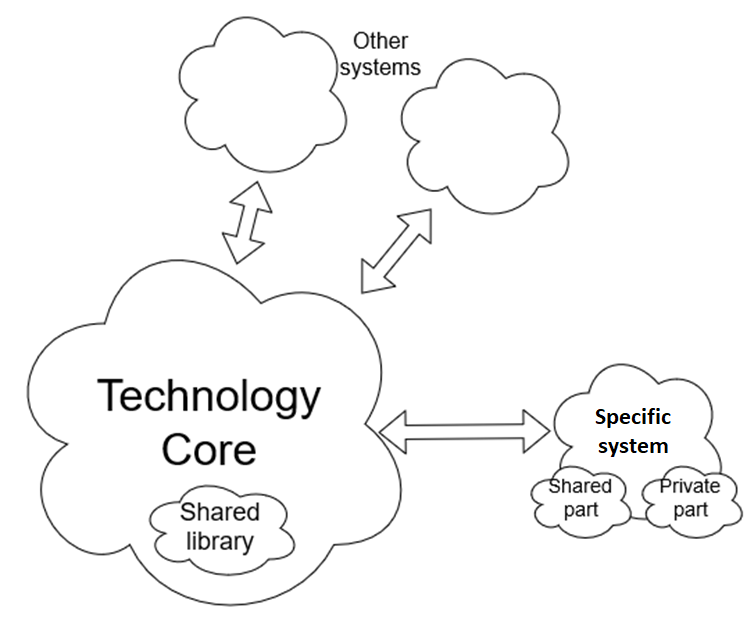
\includegraphics[width=0.6\textwidth]{figures/chapter0/ecosystem.png}}

\scnheader{Технология OSTIS}
\scnrelfromvector{текущие проекты}{Проект Экосистема OSTIS;Проект Метасистема IMS.ostis;Проект Семейство различных вариантов реализации универсального интерпретатора семантических моделей интеллектуальных систем\\
\scnaddlevel{1}
    \scnrelfromlist{подпроект}{Проект Программно реализованный на современных компьютерах универсальный интерпретатор семантических моделей интеллектуальных систем;Проект Семантический ассоциативный компьютер}
\scnaddlevel{-1}
;Проект Комплекс совместимых средств проектирования интеллектуальных систем\\
\scnaddlevel{1}
    \scnrelfromlist{подпроект}{Проект Встраиваемая типовая интеллектуальная система комплексной поддержки проектирования баз знаний;Проект Интеллектуальная система комплексной поддержки проектирования решателей задач интеллектуальных систем;Проект Интеллектуальная система комплексной поддержки проектирования вербальных интерфейсов интеллектуальных систем;Проект Интеллектуальная система комплексной поддержки проектирования невербальных интерфейсов}
\scnaddlevel{-1}
;Проект Семейство совместимых интеллектуальных справочных, обучающих и help-систем\\
\scnaddlevel{1}
    \scnrelfromlist{подпроект}{Проект Специализированные средства разработки совместимых интеллектуальных справочных, обучающих и help-систем различного назначения;Проект Комплекс семантически совместимых интеллектуальных справочных и обучающих систем по всем дисциплинам среднего образования;Проект Комплекс семантически совместимых интеллектуальных справочных и обучающих систем по всем дисциплинам, являющихся базовыми при подготовке инженеров по информационным специальностям;Проект Комплекс семантически совместимых интеллектуальных справочных и обучающих систем по всем специальным дисциплинам специальности ''Искусственный интеллект''{};Проект Семейство совместимых интеллектуальных справочных и обучающих систем по стандартам различного вида}
\scnaddlevel{-1}
;Проект Семейство совместимых интеллектуальных корпоративных систем ситуационного управления\\
\scnaddlevel{1}
    \scnrelfromlist{подпроект}{Проект Интеллектуальная корпоративная система ситуационного управления предприятием рецептурного производства;Проект Интеллектуальная корпоративная система ситуационного управления деятельностью выпускающей кафедры технического вуза}
\scnaddlevel{-1}
}
\scnrelfromvector{будущие проекты}{
Проект Семейство совместимых интеллектуальных систем автоматизации проектирования в различных областях;Проект Семейство совместимых порталов знаний\\
\scnaddlevel{1}
    \scnrelfrom{подпроект}{Проект Портал научных знаний по искусственному интеллекту}
\scnaddlevel{-1}
;Проект Семейство совместимых интеллектуальных систем экскурсионного обслуживания;Проект Семейство совместимых интеллектуальных геоинформационных систем;Проект Семейство совместимых интеллектуальных робототехнических систем и специализированных средств их разработки;Проект Семейство совместимых интеллектуальных систем персонального обслуживания и мониторинга\\
\scnaddlevel{1}
    \scnrelfromlist{подпроект}{Проект Интеллектуальная система персонального обслуживания и мониторинга пользователей и разработчиков компьютерных систем, входящих в Экосистему OSTIS;Проект Интеллектуальный персональный ассистент по взаимодействию с традиционными internet-системами и их пользователями;Проект Интеллектуальная система персонального комплексного медицинского мониторинга и контроля}
\scnaddlevel{-1}
}
\scnsegmentheader{Текущее состояние и проблемы дальнейшего развития деятельности в области Искусственного интеллекта}
\scnstartsubstruct

\scntext{аннотация}{Рассмотрим в каких направлениях должна происходить эволюция повышенного качества деятельности в области \textit{Искусственного интеллекта}, а также эволюция продуктов этой деятельности}

\bigskip
\scnfragmentcaption

\scnheader{Научно-исследовательская деятельность в области Искусственного интеллекта}
\scntext{текущее состояние}{}
\scnauthorcomment{добавить из статей}

\scnheader{Научно-исследовательская деятельность в области Искусственного интеллекта}
\scnrelfromset{проблемы текущего состояния}{
\scnfileitem{Отсутствует согласованность систем \textit{понятий} в разных направлениях \textit{Искусственного интеллекта} и, как следствие, отсутствует \textit{семантическая совместимость} и \textit{конвергенция} этих направлений, в результате чего ни о каком движении в направлении построения \textit{общей теории интеллектуальных систем} с высоким уровнем формализации и речи быть не может. Существование и продолжающееся увеличение "высоты барьеров"{} между различными направлениями исследований в области \textit{Искусственного интеллекта} проявляется в том, что специалист, работающий в рамках какого-либо направления \textit{Искусственного интеллекта}, посещая заседания "не своей"{} секции на конференции по \textit{Искусственному интеллекту}, мало что там может понять и, соответственно, извлечь полезного для себя.};
\scnfileitem{Отсутствует мотивация и осознание острой необходимости в указанной \textit{конвергенции} между различными направлениями \textit{Искусственного интеллекта}.};
\scnfileitem{Отсутствует реальное движение в направлении построения \textit{Общей теории интеллектуальных систем}, поскольку отсутствует соответствующая мотивация и осознание острой практической необходимости в этом.}
}

\bigskip
\scnfragmentcaption

\scnheader{Разработка базовой комплексной технологии проектирования интеллектуальных компьютерных систем}
\scntext{текущее состояние}{Современная технология \textit{Искусственного интеллекта} представляет собой целое семейство всевозможных частных технологий, ориентированных на разработку и сопровождение различного вида компонентов \textit{интеллектуальных компьютерных систем}, реализующих самые различные модели представления и обработки информации, различные модели решения задач, ориентированных на разработку различных классов \textit{интеллектуальных компьютерных систем}.}
\scnrelfromset{проблемы текущего состояния}{
\scnfileitem{высокая трудоемкость разработки интеллектуальных компьютерных систем};
\scnfileitem{необходимая высокая квалификация разработчиков};
\scnfileitem{современные технологии \textit{Искусственного интеллекта} принципиально не обеспечивают разработки таких \textit{интеллектуальных компьютерных систем}, в которых устраняются недостатки современных \textit{интеллектуальных компьютерных систем}};
\scnfileitem{совместимость частных технологий \textit{Искусственного интеллекта} практически отсутствует и, как следствие, отсутствует \textit{семантическая совместимость} разрабатываемых \textit{интеллектуальных компьютерных систем}, поэтому их системная интеграция осуществляется \uline{вручную}.};
\scnfileitem{Разрабатываемые \textit{интеллектуальные компьютерные системы} не способны \uline{самостоятельно} координировать свою деятельность друг с другом следовательно
\begin{scnitemize}
\item{нет общей комплексной технологии проектирования интеллектуальных компьютерных систем};
\item{не обеспечивается совместимость и взаимодействие разрабатываемых систем (синтаксическая и семантическая совместимость)};
\item{нет совместимости между существующими частными технологиями проектирования различных компонентов интеллектуальных компьютерных систем (базы знаний, нейросетевые модели, интеллектуальные интерфейсы и т.д.)};
\item{есть инструментальные средства по компонентам, но "склеивать"{} (соединять, интегрировать) это надо вручную};
\item{нет системы инструментальных средств}
\end{scnitemize}
}
}

\bigskip
\scnfragmentcaption

\scnheader{Разработка технологии производства спроектированных интеллектуальных компьютерных систем}
\scntext{текущее состояние}{Был сделан целый ряд попыток разработки \textit{компьютеров} нового поколения, ориентированных на использование в \textit{интеллектуальных компьютерных системах}. Но все они оказались неудачными, так как не были ориентированы на всё многообразие моделей решения задач в \textit{интеллектуальных компьютерных системах}. В этом смысле они не были \textit{\uline{универсальными} компьютерами} для \textit{интеллектуальных компьютерных систем}.}
\scnrelfromset{проблемы текущего состояния}{
\scnfileitem{Разрабатываемые \textit{интеллектуальные компьютерные системы} могут использовать самые различные комбинации \textit{моделей решения интеллектуальных задач} (логических моделей, соответствующих различного вида логикам, нейросетевых моделей различного вида, моделей целеполагания, синтеза планов, моделей управления сложными объектами, моделей понимания и синтеза текстов естественного языка и т.д.). Современные (традиционные, фон-неймановские) \textit{компьютеры} не в состоянии достаточно производительно интерпретировать всё многообразие указанных моделей решения задач. При этом разработка специализированных \textit{компьютеров}, ориентированных на интерпретацию какой-либо одной модели решения задач (нейросетевой модели или какой-либо логической модели) проблему не решает, так как в \textit{интеллектуальной компьютерной системе} необходимо использовать сразу несколько разных моделей решения задач, причём в различных сочетаниях.}
}

\bigskip
\scnfragmentcaption

\scnheader{Специализированная инженерия в области Искусственного интеллекта}
\scnidtf{Деятельность, направленная на разработку \textit{интеллектуальных компьютерных систем} различного назначения с использованием имеющихся для этого моделей, методов и средств}
\scnidtf{Деятельность по проектированию и производству \textit{интеллектуальных компьютерных систем}}
\scnidtf{Деятельность, направленная на формирование рынка \textit{интеллектуальных компьютерных систем}}
\scnrelfrom{в перспективе}{Специализированная инженерия в области \textit{Искусственного интеллекта}, осуществляемая специальной частью Экосистемы OSTIS}
	\scnaddlevel{1}
	\scnrelfrom{продукт}{Экосистема OSTIS}
	\scnrelfrom{субъект действия}{часть Экосистемы OSTIS, осуществляющая специализированную инженерию в области \textit{Искусственного интеллекта}}
	\scnaddlevel{-1}

\scntext{текущее состояние}{}
\scnauthorcomment{добавить из статей}

\scnrelfromset{проблемы текущего состояния}{
\scnfileitem{Отсутствует четкая систематизация многообразия \textit{интеллектуальных компьютерных систем}, соответствующая систематизации автоматизируемых \textit{видов человеческой деятельности}.};
\scnfileitem{Отсутствует \textit{конвергенция} \scnbigspace \textit{интеллектуальных компьютерных систем}, обеспечивающих автоматизацию \textit{областей человеческой деятельности}, принадлежащих одному и тому же \textit{виду человеческой деятельности}.};
\scnfileitem{Отсутствует \textit{семантическая совместимость}(семантическая унификация, взаимопонимание) между \textit{интеллектуальными компьютерными системами}, основной причиной чего является отсутствие согласованной системы общих используемых \textit{понятий}.};
\scnfileitem{Семантическая недружественность \textit{пользовательского интерфейса} и отсутствие встроенной справочной системы, позволяющей запрашивать информацию об элементах интерфейса и возможностях системы, приводят к низкой эффективности эксплуатации всех возможностей \textit{интеллектуальной компьютерной системы}.};
\scnfileitem{Анализ проблем автоматизации всех \textit{видов человеческой деятельности} убеждает в том, что дальнейшая автоматизация \textit{человеческой деятельности} требует не только повышения уровня \textit{интеллекта} соответствующих \textit{интеллектуальных компьютерных систем}, но и реализации их способности
\begin{scnitemize}
\item устанавливать свою \textit{семантическую совместимость} (взаимопонимание) как с другими \textit{компьютерными системами}, так и со своими пользователями\char59
\item поддерживать эту \textit{семантическую совместимость} в процессе собственной эволюции, а также эволюции пользователей и других \textit{компьютерных систем}\char59
\item координировать свою деятельность с пользователями и другими \textit{компьютерными системами} при коллективно решении различных задач\char59
\item участвовать в распределении работ (подзадач) при коллективном решении различных задач.
\end{scnitemize}
Важно подчеркнуть то, что реализация вышеперечисленных способностей создаст возможность для существенной и даже полной автоматизации \textit{системной интеграции} \scnbigspace \textit{компьютерных систем} в комплексы взаимодействующих систем и автоматизации реинжиниринга таких комплексов. Такая автоматизация системной интеграции и её реинжиниринга:
\begin{scnitemize}
\item даст возможность комплексам кибернетических систем \uline{самостоятельно} адаптироваться к решению новых задач\char59
\item существенно повысит эффективность эксплуатации таких комплексов компьютерных систем, так как реинжиниринг системной интеграции компьютерных систем, входящих в такой комплекс, часто востребован (например, при реконструкции предприятия)\char59
\item существенно сокращает число ошибок по сравнению с "ручным"{} (неавтоматизированным) выполнением \textit{системной интеграции} и её \textit{реинжиниринга}, которые, к тому же, требует высокой квалификации.
\end{scnitemize}
Таким образом следующий этап повышения уровня автоматизации \textit{человеческой деятельности} настоятельно требует создания таких \textit{интеллектуальных компьютерных систем}, которые могли бы легко сами (без системного интегратора) объединяться для совместного решения сложных задач. 
}
}

\bigskip
\scnfragmentcaption

\scnheader{Образовательная деятельность в области искусственного интеллекта}
\scntext{текущее состояние}{Целенаправленная подготовка специалистов в области Искусственного интеллекта имеет богатую историю и осуществляется во многих ведущих университетах (Stanford University, MIT, МГУ (Москва), НИУ МЭИ (Москва), РГГУ (Москва), СПбГУ (Санкт-Петербург), ДВФУ (Владивосток), НГТУ (Новосибирск), НТУУ КПИ (Киев), БГУИР (Минск), БГУ (Минск), БрГТУ (Брест) и других).}
\scnrelfromset{проблемы текущего состояния}{
\scnfileitem{Поскольку деятельность в области \textit{Искусственного интеллекта} сочетает в себе и высокую степень наукоемкости и высокую степень сложности инженерных работ, подготовка специалистов в этой области требует одновременного формирования у них как научно-исследовательских навыков, культуры и стиля мышления, так и инженерно-практических навыков, культуры и стиля мышления. С точки зрения методики и психологии обучения сочетание фундаментальной научной и инженерно-практической подготовки специалистов является весьма сложный образовательной педагогической задачей.};
\scnfileitem{Отсутствует \textit{семантическая совместимость} между различными учебными дисциплинами, что приводит к "мозаичности"{} восприятия информации};
\scnfileitem{Отсутствует системный подход к подготовке молодых специалистов в области \textit{Искусственного интеллекта}};
\scnfileitem{Нет персонификации обучения};
\scnfileitem{Нет установки на выявление, раскрытие и развитие таланта творческого проектирования};
\scnfileitem{Отсутствует целенаправленное формирование мотивации к творчеству};
\scnfileitem{Нет формирования навыков работы в реальных коллективах разработчиков};
\scnfileitem{Отсутствует адаптация к реальной практической деятельности};
\scnfileitem{Любая современная технология (в том числе и Технология OSTIS) должна иметь высокие темпы своего развития, поскольку без этого невозможно поддерживать высокий уровень её конкурентоспособности. Но для быстро развиваемой технологии требуется:
\begin{scnitemize}
\item не просто высокая квалификация кадров, использующих и развивающих технологию,
\item но и высокие \uline{темпы} повышения уровня этой квалификации, так как без этого невозможно эффективно использовать и развивать \uline{быстро меняющуюся} технологию.
\end{scnitemize}
\bigskip
Из этого следует, что образовательная деятельность в области \textit{Искусственного интеллекта} и соответствующая ей технология должна быть не просто важной частью деятельности в области \textit{Искусственного интеллекта}, а частью, глубоко интегрированной во все остальные виды деятельности в области \textit{Искусственного интеллекта}. Так, например, каждая \textit{интеллектуальная компьютерная система} должная быть ориентирована не только на обслуживание своих конечных пользователей, не только на организацию целенаправленного взаимодействия со своими разработчиками, которые постоянно совершенствуют эту систему, и не только на обеспечение минимального "порога вхождения"{} для новых конечных пользователей и разработчиков, но и на организацию постоянного и персонифицированного повышения квалификации каждого своего конечного пользователя и разработчика в условиях постоянных изменений, вносимых в указанную \textit{интеллектуальную компьютерную систему}. Для этого эксплуатируемая \textit{интеллектуальная компьютерная система} должна "знать"{}, что в ней изменилось, на что она способна и как эти способности инициировать (содержание и форма, соответствующих пользовательских команд)
}
}

\scnendstruct
\scnendstruct

\end{SCn}
